\subsection{Gas Experiments}

The gaseous xenon system consists of three sections.  The first section, the xenon space, contains a xenon purifier which uses hot zirconium to remove the CH$_3$T, two xenon storage bottles used to move xenon through the system via cryopumping, and a proportional tube used to detect activity within the xenon space.  The second section is a small transfer system which is used to inject consistent amounts of CH$_3$T into the xenon space with each injection.  The final section consists of a CH$_3$T storage bottle used as the source of injections and a SAES MC1-905F methane purifier to remove unwanted contaminates prior to entering the xenon space.


\begin{figure}
\centering
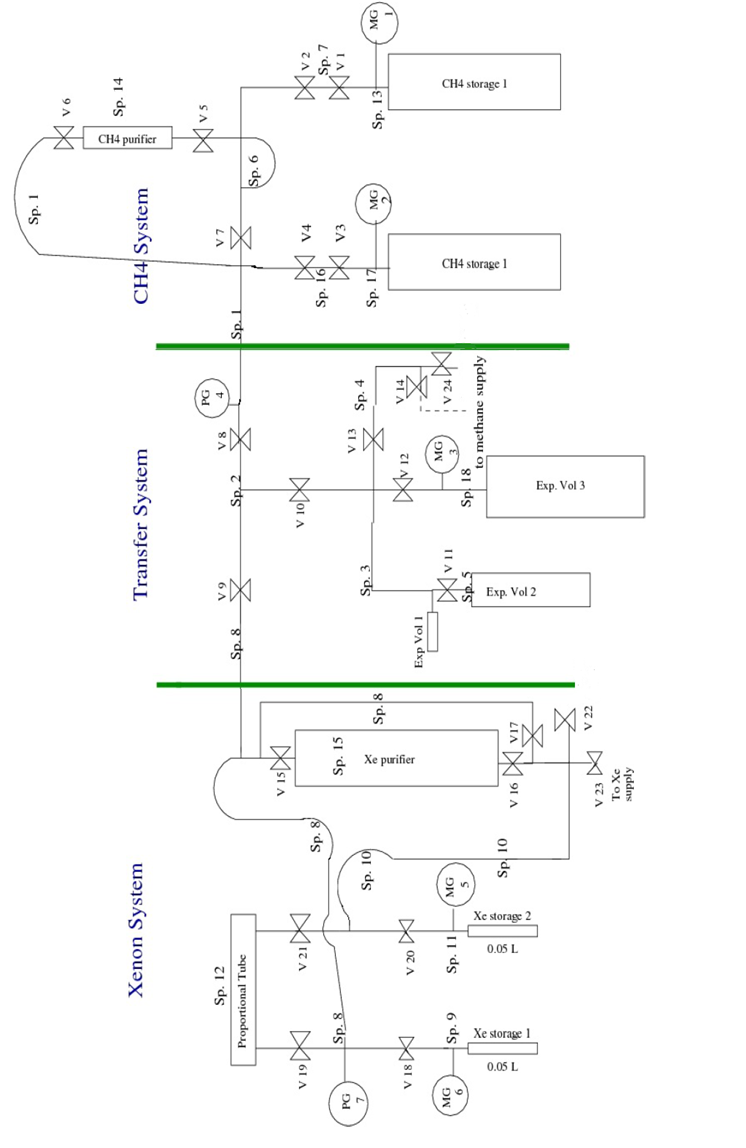
\includegraphics[scale=0.3]{GasSystem.png}
\caption{CH$_3$T gas system at UMD.  Three sections of the system are distinguished with green lines. Circles labeled PG and MG are pressure gauges, and the hourglass shapes represent hand valves.}
\label{fig:GasSys}
\end{figure}

The primary goal of this experiment was to determine the purification efficiency and study residual contamination.  There are two factors that dominate purification efficiency -- flow rate through the purifier and rest time between subsequent purifications.  High flow rates through the purifier can cool the zirconium inside, while inadequate rest time between purifications can lead to build up of methane on the surface of the zirconium beads.  Both of these situations lead to a decrease in purifier efficiency. 

The first black data point in Figure \ref{fig:InEff} is our worst purification efficiency, (96\% +/- 1\%) corresponding to our highest flow rate. (8 SLPM compared to the typical ~0.3 SLPM)  While we were unable to control the flow through our experiment as much as we desired, we are at least able to conclude that exceeding the maximum flow rate suggested for the purifier does significantly decrease purification efficiency.


\begin{figure}[H]
\caption{Single pass inefficiency of the purifier when removing CH$_3$T.  The red and blue points indicate data taken by different students, while the black points indicate data for which the procedures were intentionally altered. }
\centering
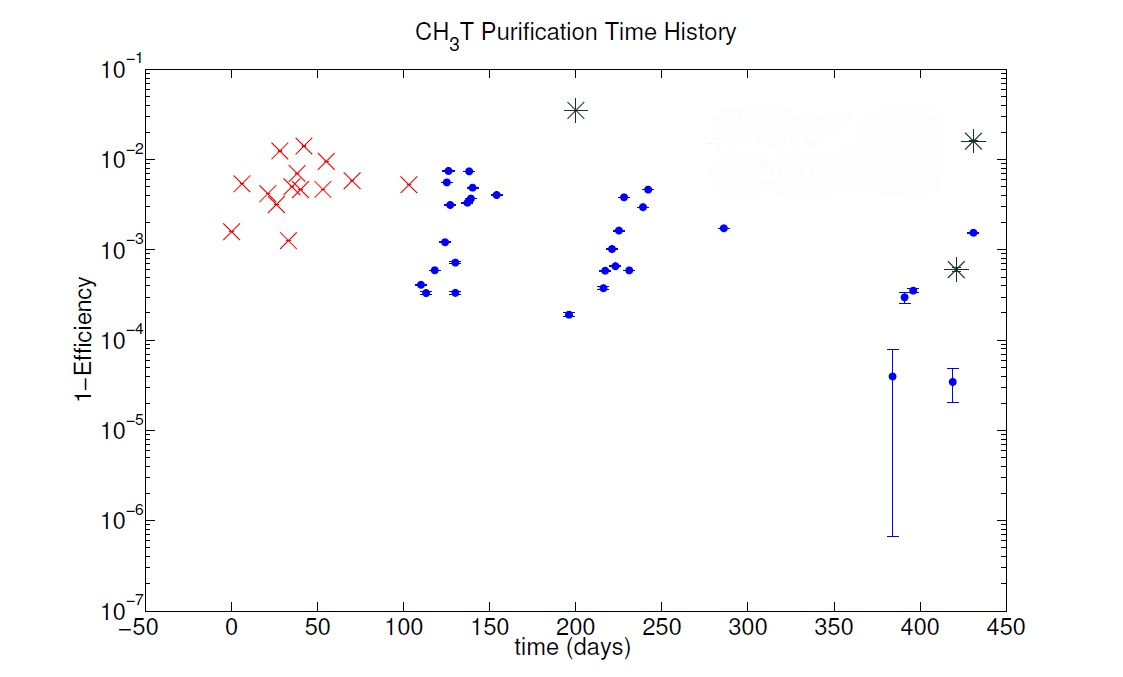
\includegraphics[scale=0.2]{Figone.png}
\label{fig:InEff}
\end{figure}


We found that allowing for ample rest time between purifications does significantly increase purification efficiency. Our best purifications were the first data points in each cluster in Figure \ref{fig:Clusters}.  We were able to obtain efficiencies of 99.99\% when the purifier was resting for three weeks or longer, and obtained efficiencies of 99\% to 99.9\% when the purifier was used on a daily basis.

\begin{figure}[H]
\centering
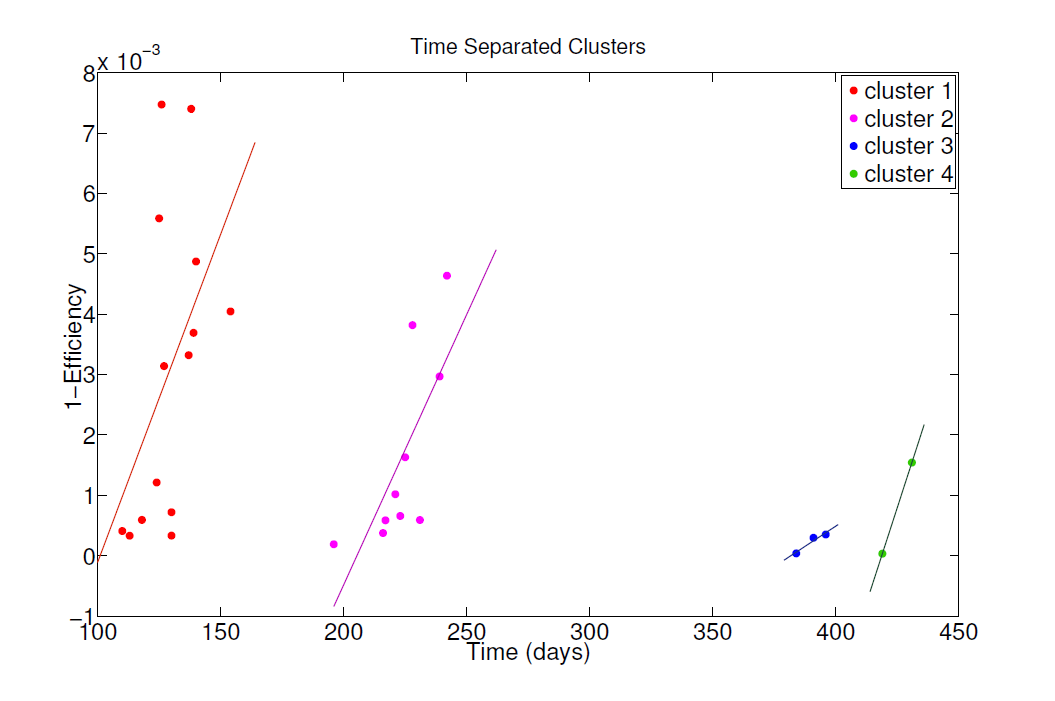
\includegraphics[scale=0.2]{Figfour.png}
\caption{Time-separated clusters of purifications have an upward trend in purification inefficiency.  Each cluster shown is separated in time by at least three weeks.}
\label{fig:Clusters}
\end{figure}

